\section{Kernel Debugging}

\subsection{Preventing bugs}

\begin{frame}[fragile]
  \frametitle{Static code analysis}
  \begin{itemize}
    \item Static analysis can be run with the {\em sparse} tool
    \item {\em sparse} works with annotation and can detect various errors at
          compile time
    \begin{itemize}
      \item Locking issues (unbalanced locking)
      \item Address space issues, such as accessing user space pointer directly
    \end{itemize}
    \item Analysis can be run using \code{make C=2} to run only on files that are
          recompiled
    \item Or with \code{make C=1} to run on all files
    \item Example of an unbalanced locking scheme:
  \end{itemize}
  \begin{block}{}
    \begin{minted}[fontsize=\small]{console}
rzn1_a5psw.c:81:13: warning: context imbalance in 'a5psw_reg_rmw' - wrong count
  at exit
    \end{minted}
  \end{block}

  \vspace{0.5cm}
  \begin{center}
    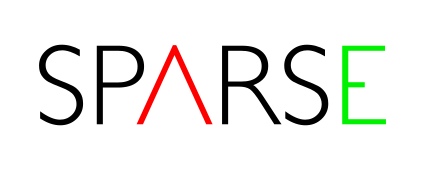
\includegraphics[height=0.1\textheight]{slides/debugging-kernel-debugging/sparse.pdf}
  \end{center}
\end{frame}

\begin{frame}[fragile]
  \frametitle{Good practices in kernel development (1/2)}
  \begin{itemize}
    \item When writing driver code, never expect the user to provide correct
          values. Always check these values.
    \item Use the \kfunc{WARN_ON} macro if you want to display a stacktrace when
      a specific condition did happen.
    \begin{itemize}
      \item \kfunc{dump_stack} can also be used during debugging to
        show the current call stack.
    \end{itemize}
  \end{itemize}
  \begin{block}{}
    \begin{minted}[fontsize=\small]{C}
static bool check_flags(u32 flags)
{
  if (WARN_ON(flags & STATE_INVALID))
    return -EINVAL;
  return 0;
}
    \end{minted}
  \end{block}
\end{frame}

\begin{frame}[fragile]
  \frametitle{Good practices in kernel development (2/2)}
  \begin{itemize}
    \item If the values can be checked at compile time (configuration input,
          \kfunc{sizeof} structure fields), use the \kfunc{BUILD_BUG_ON} macro to
          ensure the condition is true.
  \end{itemize}
  \begin{block}{}
    \begin{minted}[fontsize=\small]{C}
BUILD_BUG_ON(sizeof(ctx->__reserved) != sizeof(reserved));
    \end{minted}
  \end{block}
  \begin{itemize}
    \item If during compilation you have some warnings about unused
          variables/parameters, they must be fixed.
    \item Apply \code{checkpatch.pl --strict} when possible which might find some
          potential problems in your code.
  \end{itemize}
\end{frame}

\subsection{Linux Kernel Debugging}

\begin{frame}
  \frametitle{Linux Kernel Debugging}
  \begin{itemize}
    \item The Linux Kernel features some very useful tools for debugging.
    \item These tools are builtin the kernel since their activation often
          selects instrumentation code for debugging
    \begin{itemize}
      \item Erroneous memory accesses debugging tools ({\em KASAN}, {\em Kmemleak}, {\em KFENCE})
      \item Undefined behavior code debugging ({\em UBSAN})
      \item Locking errors analysis ({\em lockdep})
    \end{itemize}
    \item All the debug features are located under the \code{Kernel hacking ->
          Kernel debugging} menuconfig entry.
    \begin{itemize}
    \item \kconfig{CONFIG_DEBUG_KERNEL} should be set to "y" to enable other
          debug options.
    \end{itemize}
  \end{itemize}
\end{frame}

\subsection{Debugging using messages}

\begin{frame}[fragile]
  \frametitle{Debugging using messages (1/3)}
  Three APIs are available
  \begin{itemize}
  \item The old \kfunc{printk}, no longer recommended for new debugging
    messages
  \item The \code{pr_*()} family of functions: \kfunc{pr_emerg},
    \kfunc{pr_alert}, \kfunc{pr_crit}, \kfunc{pr_err},
    \kfunc{pr_warning}, \kfunc{pr_notice}, \kfunc{pr_info},
    \kfunc{pr_cont} \\
    and the special \kfunc{pr_debug} (see next pages)
    \begin{itemize}
    \item Defined in \kfile{include/linux/printk.h}
    \item They take a classic format string with arguments
    \item Example:
      \begin{minted}{c}
pr_info("Booting CPU %d\n", cpu);
      \end{minted}
    \item Here's what you get in the kernel log:
      \begin{verbatim}
[  202.350064] Booting CPU 1
      \end{verbatim}
    \end{itemize}
    \item \kfunc{print_hex_dump_debug}: useful to dump a buffer with
      \code{hexdump} like display
  \end{itemize}
\end{frame}

\begin{frame}[fragile]
  \frametitle{Debugging using messages (2/3)}
  \begin{itemize}
  \item The \code{dev_*()} family of functions: \kfunc{dev_emerg},
    \kfunc{dev_alert}, \kfunc{dev_crit}, \kfunc{dev_err},
    \kfunc{dev_warn}, \kfunc{dev_notice}, \kfunc{dev_info} \\
    and the special \kfunc{dev_dbg} (see next page)
    \begin{itemize}
    \item They take a pointer to \kstruct{device} as first
      argument, and then a format string with arguments
    \item Defined in \kfile{include/linux/dev_printk.h}
    \item To be used in drivers integrated with the Linux device
      model
    \item Example:
      \begin{minted}{c}
dev_info(&pdev->dev, "in probe\n");
      \end{minted}
    \item Here's what you get in the kernel log:
      \begin{verbatim}
[   25.878382] serial 48024000.serial: in probe
[   25.884873] serial 481a8000.serial: in probe
      \end{verbatim}
    \end{itemize}
  \item \code{*_ratelimited()} version exists which limits the amount of print
    if called too much based on \code{/proc/sys/kernel/printk_ratelimit{_burst}}
    values
  \end{itemize}
\end{frame}

\begin{frame}[fragile]
  \frametitle{Debugging using messages (3/3)}
  \begin{itemize}
  \item The kernel defines many more format specifiers than the standard
    \code{printf()} existing ones.
  \begin{itemize}
    % \path of package url directly supports percent characters, unless it is
    % used inside arguments of other macros which is the case of the \code macro
    \item {\codecolor \path{%p}}: Display the hashed value of pointer by default.
    \item {\codecolor \path{%px}}: Always display the address of a pointer (use
      carefully on non-sensitive addresses).
    \item {\codecolor \path{%pK}}: Display hashed pointer value, zeros or the
      pointer address depending on \code{kptr_restrict} sysctl value.
    \item {\codecolor \path{%pOF}}: Device-tree node format specifier.
    \item {\codecolor \path{%pr}}: Resource structure format specifier.
    \item {\codecolor \path{%pa}}: Physical address display (work on all architectures 32/64
      bits)
    \item {\codecolor \path{%pe}}: Error pointer (displays the string
      corresponding to the error number)
  \end{itemize}
  \item \code{/proc/sys/kernel/kptr_restrict} should be set to \code{1} in order
    to display pointers which uses {\codecolor \path{%pK}}
  \item See \kdochtml{core-api/printk-formats} for an exhaustive list of supported format
    specifiers
  \end{itemize}
\end{frame}

\begin{frame}
  \frametitle{pr\_debug() and dev\_dbg()}
  \begin{itemize}
  \item When the driver is compiled with \code{DEBUG} defined, all
    these messages are compiled and printed at the debug level.
    \code{DEBUG} can be defined by \codewithhash{\#define DEBUG} at the
    beginning of the driver, or using
    \code{ccflags-$(CONFIG_DRIVER) += -DDEBUG} in the \code{Makefile}
  \item When the kernel is compiled with \kconfig{CONFIG_DYNAMIC_DEBUG},
    then these messages can dynamically be enabled on a per-file,
    per-module or per-message basis
    \begin{itemize}
    \item Details in \kdochtml{admin-guide/dynamic-debug-howto}
    \item Very powerful feature to only get the debug messages you're
      interested in.
    \end{itemize}
  \item When neither \code{DEBUG} nor \kconfig{CONFIG_DYNAMIC_DEBUG} are
    used, these messages are not compiled in.
  \end{itemize}
\end{frame}

\ifthenelse{\equal{\training}{debugging}}{
\begin{frame}
  \frametitle{pr\_debug() and dev\_dbg() usage}
  \begin{itemize}
  \item Debug prints can be enabled using the
    \code{/sys/kernel/debug/dynamic_debug/control} file.
  \begin{itemize}
    \item \code{cat /sys/kernel/debug/dynamic_debug/control} will display all
      lines that can be enabled in the kernel
    \item Example: \code{init/main.c:1427 [main]run_init_process =p "    \%s\012"}
  \end{itemize}
  \item A syntax allows to enable individual print using lines, files or modules
  \begin{itemize}
    \item \code{echo "file drivers/pinctrl/core.c +p" > /sys/kernel/debug/dynamic_debug/control}
      will enable all debug prints in \code{drivers/pinctrl/core.c}
    \item \code{echo "module pciehp +p" > /sys/kernel/debug/dynamic_debug/control}
      will enable the debug print located in the \code{pciehp} module
    \item \code{echo "file init/main.c line 1427 +p" > /sys/kernel/debug/dynamic_debug/control}
      will enable the debug print located at line 1247 of file \code{init/main.c}
    \item Replace \code{+p} with \code{-p} to disable the debug print
  \end{itemize}
  \end{itemize}
\end{frame}
}{}

\ifthenelse{\equal{\training}{linux-kernel}}{
\begin{frame}
  \frametitle{Configuring the priority}
  \begin{itemize}
  \item Each message is associated to a priority, ranging from \code{0} for
    emergency to \code{7} for debug, as specified in
    \kfile{include/linux/kern_levels.h}.
  \item All the messages, regardless of their priority, are stored in
    the kernel log ring buffer
    \begin{itemize}
    \item Typically accessed using the \code{dmesg} command
    \end{itemize}
  \item Some of the messages may appear on the console, depending on
    their priority and the configuration of
    \begin{itemize}
    \item The \code{loglevel} kernel parameter, which defines the
      priority number below which messages are displayed on the console.
      Details in \kdochtml{admin-guide/kernel-parameters}.
      \newline Examples: \code{loglevel=0}: no message, \code{loglevel=8}: all messages
    \item The value of \code{/proc/sys/kernel/printk}, which allows to
      change at runtime the priority above which messages are
      displayed on the console. Details in
      \kdochtml{admin-guide/sysctl/kernel}
    \end{itemize}
  \end{itemize}
\end{frame}
}{}

\ifthenelse{\equal{\training}{debugging}}{
\begin{frame}
  \frametitle{Debug logs troubleshooting}
  \begin{itemize}
    \item Make sure that your debug call is enabled: it must be visible in
    \code{control} file in debugfs \textbf{and} be actived (\code{=p})
    \item Is your log output only in kernel log buffer ?
    \begin{itemize}
      \item You can see it thanks to \code{dmesg}
      \item You can lower \code{loglevel} to output it to console directly
      \item You can also set \code{ignore_loglevel} in kernel command line to
      force all kernel logs to console
    \end{itemize}
    \item If you are working on an out-of-tree module, you may prefer to define \code{DEBUG} in
    your module source or Makefile instead of using dynamic debug
    \item If configuration is done through kernel commandline, is it
    properly interpreted ?
    \begin{itemize}
      \item Starting from 5.14, kernel will let you know about faulty
      commandline:\\
      \code{Unknown kernel command line parameters foo, will be passed to user
      space.}
      \item You may need to take care of special characters escaping (e.g: quotes)
    \end{itemize}
  \end{itemize}
\end{frame}
}{}

\begin{frame}
  \frametitle{Kernel early debug}
  \begin{itemize}
  \item When booting, the kernel sometimes crashes even before displaying
    the system messages
  \item On ARM, if your kernel doesn't boot or hangs without any
    message, you can activate early debugging options
  \begin{itemize}
    \item \kconfigval{CONFIG_DEBUG_LL}{y} to enable ARM early serial output
      capabilities
    \item \kconfigval{CONFIG_EARLYPRINTK}{y} will allow printk to output the
      prints earlier
  \end{itemize}
  \item \code{earlyprintk} command line parameter should be given to enable
    early printk output
  \end{itemize}
\end{frame}

\subsection{Kernel crashes and oops}

\begin{frame}
  \frametitle{Kernel crashes}
  \begin{itemize}
    \item The kernel is not immune to crash, many errors can be done and lead to
          crashes
    \begin{itemize}
      \item Memory access error (NULL pointer, out of bounds access, etc)
      \item Voluntarily panicking on error detection (using \kfunc{panic})
      \item Kernel incorrect execution mode (sleeping in atomic context)
      \item Deadlocks detected by the kernel (Soft lockup/locking problem)
    \end{itemize}
    \item On error, the kernel will display a message on the console that
          is called a "Kernel oops"
  \end{itemize}
  \begin{center}
    \center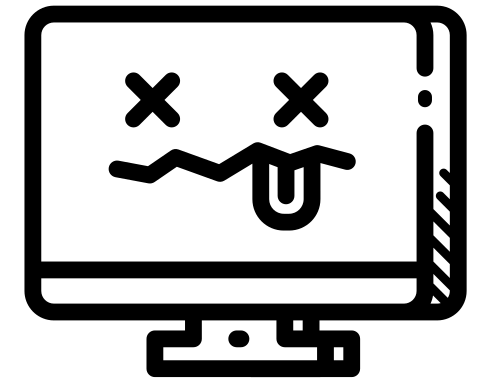
\includegraphics[height=0.3\textheight]{slides/debugging-kernel-debugging/crash.png}\\
    {\tiny {\em Icon by Peter van Driel, TheNounProject.com}}
  \end{center}
\end{frame}

\begin{frame}
  \frametitle{Kernel oops (1/2)}
  \begin{itemize}
    \item The content of this message depends on the architecture that is used.
    \item Almost all architectures display at least the following information:
    \begin{itemize}
      \item CPU state when the oops happened
      \item Registers content with potential interpretation
      \item Backtrace of function calls that led to the crash
      \item Stack content (last X bytes)
    \end{itemize}
    \item Depending on the architecture, the crash location can be identified
          using the content of the PC registers (sometimes named IP, EIP, etc).
    \item To have a meaningful backtrace with symbol names use
          \kconfigval{CONFIG_KALLSYMS}{y} which will embed the
          symbol names in the kernel image.
  \end{itemize}
\end{frame}

\begin{frame}
  \frametitle{Kernel oops (2/2)}
  \begin{itemize}
    \item Symbols are displayed in the backtrace using the following format:
    \begin{itemize}
      \item \code{<symbol_name>+<hex_offset>/<symbol_size>}
    \end{itemize}
    \item If the oops is not critical (taken in process context), then the
          kernel will kill process and continue its execution
    \begin{itemize}
      \item The kernel stability might be compromised!
    \end{itemize}
    \item Tasks that are taking too much time to execute and that are hung can
          also generate an oops (\kconfig{CONFIG_DETECT_HUNG_TASK})
    \item If KGDB support is present and configured, on oops, the kernel will
          switch to KGDB mode.
  \end{itemize}
\end{frame}

\begin{frame}
  \frametitle{Oops example (1/2)}
  \begin{center}
    \includegraphics[height=0.8\textheight]{slides/debugging-kernel-debugging/oops1.pdf}
  \end{center}
\end{frame}

\begin{frame}
  \frametitle{Oops example (2/2)}
  \begin{center}
    \includegraphics[height=0.8\textheight]{slides/debugging-kernel-debugging/oops2.pdf}
  \end{center}
\end{frame}

\begin{frame}
  \frametitle{Kernel oops debugging: \code{addr2line}}
  \begin{itemize}
    \item In order to convert addresses/symbol name from this display to source
      code lines, one can use addr2line
    \begin{itemize}
      \item \code{addr2line -e vmlinux <address>}
    \end{itemize}
    \item GNU binutils >= 2.39 takes the symbol+offset notation too:
    \begin{itemize}
      \item \code{addr2line -e vmlinux <symbol_name>+<off>}
    \end{itemize}
    \item The symbol+offset notation can be used with older binutils
      versions via the \code{faddr2line} script in the kernel sources:
    \begin{itemize}
      \item \code{scripts/faddr2line vmlinux <symbol_name>+<off>}
    \end{itemize}
    \item The kernel must have been compiled with
      \kconfigval{CONFIG_DEBUG_INFO}{y} to embed the debugging information into
      the vmlinux file.
  \end{itemize}
\end{frame}

\begin{frame}
  \frametitle{Kernel oops debugging: \code{decode_stacktrace.sh}}
  \begin{itemize}
    \item \code{addr2line} decoding of oopses can be automated using
      \code{decode_stacktrace.sh} script which is provided in the kernel
      sources.
    \item This script will translate all symbol names/addresses to the matching
      file/lines and will display the assembly code where the crash did trigger.
    \item \code{./scripts/decode_stacktrace.sh vmlinux linux_source_path/ < oops_report.txt > decoded_oops.txt}

    \item NOTE: \code{CROSS_COMPILE} and \code{ARCH} env var should be set to
      obtain the correct disassembly dump.
  \end{itemize}
\end{frame}

\begin{frame}
  \frametitle{Oops behavior configuration}
  \begin{itemize}
    \item Sometimes, crash might be so bad that the kernel will panic and halt
          its execution entirely by stopping scheduling application and staying
          in a busy loop.
    \item Automatic reboot on panic can be enabled via
      \kconfig{CONFIG_PANIC_TIMEOUT}
    \begin{itemize}
      \item 0: never reboots
      \item Negative value: reboot immediately
      \item Positive value: seconds to wait before rebooting
    \end{itemize}
    \item OOPS can be configured to always panic:
    \begin{itemize}
      \item at boot time, adding \code{oops=panic} to the command line
      \item at build time, setting \kconfigval{CONFIG_PANIC_ON_OOPS}{y}
    \end{itemize}
  \end{itemize}
\end{frame}

\subsection{The Magic SysRq}

\begin{frame}[fragile]
  \frametitle{The Magic SysRq}
  Functionality provided by serial drivers
  \begin{itemize}
  \item Allows to run multiple debug/rescue commands even when the
    kernel seems to be in deep trouble
    \begin{itemize}
      \item On embedded: in the console, send a break character\\
        (Picocom: press \code{[Ctrl]} + \code{a} followed by \code{[Ctrl]}
        + \code{\ }), then press \code{<character>}
       \item By echoing \code{<character>} in \code{/proc/sysrq-trigger}
    \end{itemize}
  \item Example commands:
    \begin{itemize}
    \item \code{h}: show available commands
    \item \code{s}: sync all mounted filesystems
    \item \code{b}: reboot the system
    \item \code{w}: shows the kernel stack of all sleeping processes
    \item \code{t}: shows the kernel stack of all running processes
    \item \code{g}: enter kgdb mode
    \item \code{z}: flush trace buffer
    \item \code{c}: triggers a crash (kernel panic)
    \item You can even register your own!
    \end{itemize}
  \item Detailed in \kdochtml{admin-guide/sysrq}
  \end{itemize}
\end{frame}

\subsection{Built-in kernel self tests}

\begin{frame}
  \frametitle{Kernel memory issue debugging}
  \begin{itemize}
    \item The same kind of memory issues that can happen in user space can be
          triggered while writing kernel code
    \begin{itemize}
      \item Out of bounds accesses
      \item Use-after-free errors (dereferencing a pointer after \code{kfree()})
      \item Out of memory due to missing \code{kfree()}
    \end{itemize}
    \item Various tools are present in the kernel to catch these issues
    \begin{itemize}
      \item {\em KASAN} to find use-after-free and out-of-bound memory accesses
      \item {\em KFENCE} to find use-after-free and out-of-bound in production systems
      \item {\em Kmemleak} to find memory leak due to missing free of memory
    \end{itemize}
  \end{itemize}
\end{frame}

\begin{frame}
  \frametitle{{\em KASAN}}
  \begin{itemize}
    \item Kernel Address Space Sanitizer
    \item Allows to find use-after-free and out-of-bounds memory accesses
    \item Uses GCC to instrument the kernel at compile-time
    \item Supported by almost all architectures (ARM, ARM64, PowerPC, RISC-V,
          S390, Xtensa and X86)
    \item Needs to be enabled at kernel configuration with
          \kconfig{CONFIG_KASAN}
    \item Can then be enabled for files by modifying Makefile
    \begin{itemize}
      \item \code{KASAN_SANITIZE_file.o := y} for a specific file
      \item \code{KASAN_SANITIZE := y} for all files in the Makefile folder
    \end{itemize}
  \end{itemize}
\end{frame}

\begin{frame}
  \frametitle{{\em Kmemleak}}
  \begin{itemize}
    \item Kmemleak allows to find memory leaks for dynamically allocated objects
          with \code{kmalloc()}
    \begin{itemize}
      \item Works by scanning the memory to detect if allocated address are not
            referenced anymore anywhere (large overhead).
    \end{itemize}
    \item Once enabled with \kconfig{CONFIG_DEBUG_KMEMLEAK}, kmemleak control
          files will be visible in {\em debugfs}
    \item Memory leaks is scanned every 10 minutes
    \begin{itemize}
      \item can be disabled via \kconfig{CONFIG_DEBUG_KMEMLEAK_AUTO_SCAN}
    \end{itemize}
    \item An immediate scan can be triggered using 
    \begin{itemize}
      \item \codewithhash{\# echo scan > /sys/kernel/debug/kmemleak}
    \end{itemize}
    \item Results are displayed in debugfs
    \begin{itemize}
      \item \codewithhash{\# cat /sys/kernel/debug/kmemleak}
    \end{itemize}
    \item See \kdochtml{dev-tools/kmemleak} for more information
  \end{itemize}
\end{frame}

\begin{frame}[fragile]
  \frametitle{{\em Kmemleak} report}
  \begin{block}{}
    \begin{minted}[fontsize=\small]{console}
# cat /sys/kernel/debug/kmemleak
unreferenced object 0x82d43100 (size 64):
  comm "insmod", pid 140, jiffies 4294943424 (age 270.420s)
  hex dump (first 32 bytes):
    b4 bb e1 8f c8 a4 e1 8f 8c ce e1 8f 88 c6 e1 8f  ................
    10 a5 e1 8f 18 e2 e1 8f ac c6 e1 8f 0c c1 e1 8f  ................
  backtrace:
    [<c31f5b59>] slab_post_alloc_hook+0xa8/0x1b8
    [<c8200adb>] kmem_cache_alloc_trace+0xb8/0x104
    [<1836406b>] 0x7f005038
    [<89fff56d>] do_one_initcall+0x80/0x1a8
    [<31d908e3>] do_init_module+0x50/0x210
    [<2658dd55>] load_module+0x208c/0x211c
    [<e1d48f15>] sys_finit_module+0xe4/0xf4
    [<1de12529>] ret_fast_syscall+0x0/0x54
    [<7ee81f34>] 0x7eca8c80
    \end{minted}
  \end{block}
\end{frame}

\begin{frame}
  \frametitle{{\em UBSAN}}
  \begin{itemize}
    \item UBSAN is a runtime checker for code with undefined behavior
    \begin{itemize}
      \item Shifting with a value larger than the type
      \item Overflow of integers (signed and unsigned)
      \item Misaligned pointer access
      \item Out of bound access to static arrays
      \item https://clang.llvm.org/docs/UndefinedBehaviorSanitizer.html
    \end{itemize}
    \item It uses compile-time instrumentation to insert checks that will be
          executed at runtime
    \item Must be enabled using \kconfigval{CONFIG_UBSAN}{y}
    \item Then, can be enabled for specific files by modifying Makefile
    \begin{itemize}
      \item \code{UBSAN_SANITIZE_file.o := y} for a specific file
      \item \code{UBSAN_SANITIZE := y} for all files in the Makefile folder
    \end{itemize}
  \end{itemize}
\end{frame}

\begin{frame}[fragile]
  \frametitle{{\em UBSAN}: example of UBSAN report}
  \begin{itemize}
    \item Report for an undefined behavior due to a shift with a value > 32.
  \end{itemize}
  \begin{block}{}
    \begin{minted}[fontsize=\tiny]{console}
UBSAN: Undefined behaviour in mm/page_alloc.c:3117:19
shift exponent 51 is too large for 32-bit type 'int'
CPU: 0 PID: 6520 Comm: syz-executor1 Not tainted 4.19.0-rc2 #1
Hardware name: QEMU Standard PC (i440FX + PIIX, 1996), BIOS Bochs 01/01/2011
Call Trace:
__dump_stack lib/dump_stack.c:77 [inline]
dump_stack+0xd2/0x148 lib/dump_stack.c:113
ubsan_epilogue+0x12/0x94 lib/ubsan.c:159
__ubsan_handle_shift_out_of_bounds+0x2b6/0x30b lib/ubsan.c:425
...
RIP: 0033:0x4497b9
Code: e8 8c 9f 02 00 48 83 c4 18 c3 0f 1f 80 00 00 00 00 48 89 f8 48
89 f7 48 89 d6 48 89 ca 4d 89 c2 4d 89 c8 4c 8b 4c 24 08 0f 05 <48> 3d
01 f0 ff ff 0f 83 9b 6b fc ff c3 66 2e 0f 1f 84 00 00 00 00
RSP: 002b:00007fb5ef0e2c68 EFLAGS: 00000246 ORIG_RAX: 0000000000000010
RAX: ffffffffffffffda RBX: 00007fb5ef0e36cc RCX: 00000000004497b9
RDX: 0000000020000040 RSI: 0000000000000258 RDI: 0000000000000014
RBP: 000000000071bea0 R08: 0000000000000000 R09: 0000000000000000
R10: 0000000000000000 R11: 0000000000000246 R12: 00000000ffffffff
R13: 0000000000005490 R14: 00000000006ed530 R15: 00007fb5ef0e3700 
    \end{minted}
  \end{block}
\end{frame}

\begin{frame}
  \frametitle{Debugging locking}
  \begin{itemize}
  \item Lock debugging: prove locking correctness
    \begin{itemize}
    \item \kconfig{CONFIG_PROVE_LOCKING}
    \item Adds instrumentation to kernel locking code
    \item Detect violations of locking rules during system life, such as:
      \begin{itemize}
      \item Locks acquired in different order (keeps track of locking
        sequences and compares them).
      \item Spinlocks acquired in interrupt handlers and also in
        process context when interrupts are enabled.
      \end{itemize}
    \item Not suitable for production systems but acceptable overhead
      in development.
    \item See \kdochtml{locking/lockdep-design} for details
    \end{itemize}
    \item \kconfig{CONFIG_DEBUG_ATOMIC_SLEEP} allows to detect code that
      incorrectly sleeps in atomic section (while holding lock typically).
      \begin{itemize}
        \item Warning displayed in the dmesg in case of such violation.
        \end{itemize}
  \end{itemize}
\end{frame}

\begin{frame}
  \frametitle{Concurrency issues}
  \begin{itemize}
    \item Kernel Concurrency SANitizer framework
    \item \kconfig{CONFIG_KCSAN}, introduced in Linux 5.8.
    \item Dynamic race detector relying on compile time instrumentation. 
    \item Can find concurrency issues (mainly data races) in your system.
    \item See \kdochtml{dev-tools/kcsan} and
        \url{https://lwn.net/Articles/816850/} for details.
  \end{itemize}
\end{frame}


\subsection{KGDB}


\begin{frame}
  \frametitle{kgdb - A kernel debugger}
  \begin{itemize}
  \item \kconfig{CONFIG_KGDB} in {\em Kernel hacking}.
  \item The execution of the kernel is fully controlled by \code{gdb}
    from another machine, connected through a serial line.
  \item Can do almost everything, including inserting breakpoints in
    interrupt handlers.
  \item Feature supported for the most popular CPU architectures
  \item \kconfig{CONFIG_GDB_SCRIPTS} allows to build GDB python scripts that are
    provided by the kernel.
  \begin{itemize}
    \item See \kdochtml{dev-tools/gdb-kernel-debugging} for more information
  \end{itemize}
  \end{itemize}
\end{frame}

\ifthenelse{\equal{\training}{debugging}}{

\begin{frame}
  \frametitle{kgdb kernel config}
  \begin{itemize}
    \item \kconfigval{CONFIG_DEBUG_KERNEL}{y} to make KGDB support visible
    \item \kconfigval{CONFIG_KGDB}{y} to enabled KGDB support
    \item \kconfigval{CONFIG_DEBUG_INFO}{y} to enabled KGDB support
    \item \kconfigval{CONFIG_FRAME_POINTER}{y} to have more reliable
          stacktraces
    \item \kconfigval{CONFIG_KGDB_SERIAL_CONSOLE}{y} to enabled KGDB support
          over serial
    \item \kconfigval{CONFIG_GDB_SCRIPTS}{y} to enabled kernel GDB python
          scripts
    \item \kconfigval{CONFIG_RANDOMIZE_BASE}{n} and
          \kconfigval{CONFIG_WATCHDOG}{n} to disable KALSR and watchdog
    \item \kconfigval{CONFIG_MAGIC_SYSRQ} to enable Magic SysReq support
    \item \kconfigval{CONFIG_STRICT_KERNEL_RWX}{n} to disable memory protection
          on code section, thus allowing to put breakpoints
  \end{itemize}
\end{frame}

\begin{frame}
  \frametitle{kgdb pitfalls}
  \begin{itemize}
    \item KASLR should be disabled to avoid confusing gdb with randomized kernel
          addresses
    \begin{itemize}
      \item Disable \em{kaslr} mode using \code{nokaslr} command line parameter
            if enabled in your kernel.
    \end{itemize}
    \item Disable the platform watchdog to avoid rebooting while debugging.
    \begin{itemize}
      \item When interrupted by KGDB, all interrupts are disabled thus, the
            watchdog is not serviced.
      \item Sometimes, watchdog is enabled by upper boot levels. Make sure to
            disabled the watchdog there too.
    \end{itemize}
    \item Can not interrupt kernel execution from gdb using \code{interrupt}
          command or \code{Ctrl + C}.
    \item Not possible to break everywhere (see \kconfig{CONFIG_KGDB_HONOUR_BLOCKLIST}).
    \item Need a console driver with polling support.
    \item Some architecture lacks functionalities (No watchpoints on arm32 for
          instance).
  \end{itemize}
\end{frame}
}{}

\begin{frame}
  \frametitle{Using kgdb (1/2)}
  \begin{itemize}
  \item Details available in the kernel documentation:
    \kdochtml{dev-tools/kgdb}
  \item You must include a kgdb I/O driver. One of them is \code{kgdb} over
    serial console (\code{kgdboc}: \code{kgdb} over console, enabled by
    \kconfig{CONFIG_KGDB_SERIAL_CONSOLE})
  \item Configure \code{kgdboc} at boot time by passing to the kernel:
    \begin{itemize}
    \item \code{kgdboc=<tty-device>,<bauds>}.
    \item For example: \code{kgdboc=ttyS0,115200}
    \end{itemize}
  \item Or at runtime using sysfs:
   \begin{itemize}
   \item \code{echo ttyS0 > /sys/module/kgdboc/parameters/kgdboc}
   \item If the console does not have polling support, this command will yield
         an error.
   \end{itemize}
  \end{itemize}
\end{frame}

\begin{frame}
  \frametitle{Using kgdb (2/2)}
  \begin{itemize}
  \item Then also pass \code{kgdbwait} to the kernel: it makes
    \code{kgdb} wait for a debugger connection.
  \item Boot your kernel, and when the console is initialized,
    interrupt the kernel with a break character and then \code{g}
    in the serial console (see our {\em Magic SysRq} explanations).
  \item On your workstation, start \code{gdb} as follows:
    \begin{itemize}
    \item \code{arm-linux-gdb ./vmlinux}
    \item \code{(gdb) set remotebaud 115200}
    \item \code{(gdb) target remote /dev/ttyS0}
    \end{itemize}
  \item Once connected, you can debug a kernel the way you would debug
    an application program.
  \end{itemize}
\end{frame}

\begin{frame}
  \frametitle{Kernel {\em GDB} scripts}
  \begin{itemize}
    \item \kconfig{CONFIG_GDB_SCRIPTS} allows to build a set of python script
          which ease the kernel debugging by adding new commands and functions.
    \item When using \code{gdb vmlinux}, the scripts present in vmlinux-gdb.py
          file at the root of build dir will be loaded automatically.
    \begin{itemize}
      \item \code{lx-symbols}: (Re)load symbols for vmlinux and modules
      \item \code{lx-dmesg}: display kernel dmesg
      \item \code{lx-lsmod}: display loaded modules
      \item \code{lx-device-{bus|class|tree}}: display device bus, classes and
            tree
      \item \code{lx-ps}: \code{ps} like view of tasks
      \item \code{$lx_current()} contains the current \code{task_struct}
      \item \code{$lx_per_cpu(var, cpu)} returns a per-cpu variable
      \item \code{apropos lx} To display all available functions.
    \end{itemize}
    \item \kdochtml{dev-tools/gdb-kernel-debugging}
  \end{itemize}
\end{frame}

\begin{frame}
  \frametitle{{\em KDB}}
  \begin{itemize}
    \item \kconfig{CONFIG_KGDB_KDB} includes a kgdb frontend name "KDB"
    \item This frontend exposes a debug prompt on the serial console which
          allows debugging the kernel without the need for an external gdb.
    \item KDB can be entered using the same mechanism used for entering kgdb
          mode.
    \item {\em KDB} and {\em KGDB} can coexist and be used at the same time.
    \begin{itemize}
      \item Use the \code{kgdb} command in KDB to enter kgdb mode.
      \item Send a maintenance packet from gdb using \code{maintenance packet 3}
            to switch from kgdb to KDB mode.
    \end{itemize}
  \end{itemize}
\end{frame}

\begin{frame}[fragile]
  \frametitle{{\em kdmx}}
  \begin{itemize}
    \item When the system has only a single serial port, it is not possible to
          use both KGDB and the serial line as an output terminal since only one
          program can access that port.
    \item Fortunately, the {\em kdmx} tool allows to use both KGDB and serial
          output by splitting GDB messages and standard console from a single
          port to 2 slave pty (\code{/dev/pts/x})
    \item https://git.kernel.org/pub/scm/utils/kernel/kgdb/agent-proxy.git
    \begin{itemize}
      \item Located in the subdirectory \code{kdmx}
    \end{itemize}
  \end{itemize}
  \begin{columns}
    \column{0.5\textwidth}
    \begin{block}{}
      \begin{minted}[fontsize=\tiny]{console}
$ kdmx -n -d -p/dev/ttyACM0 -b115200
serial port: /dev/ttyACM0
Initalizing the serial port to 115200 8n1
/dev/pts/6 is slave pty for terminal emulator
/dev/pts/7 is slave pty for gdb

Use <ctrl>C to terminate program
      \end{minted}
    \end{block}
    \column{0.5\textwidth}
    \includegraphics[width=\textwidth]{slides/debugging-kernel-debugging/kdmx.pdf}
  \end{columns}
\end{frame}

\begin{frame}[fragile]
  \frametitle{Going further with KGDB}
  \begin{itemize}
    \item Good presentation from Doug Anderson with a lot of demos and
          explanations
    \begin{itemize}
      \item Video: \url{https://www.youtube.com/watch?v=HBOwoSyRmys}
      \item Slides: \url{https://elinux.org/images/1/1b/ELC19_Serial_kdb_kgdb.pdf}
    \end{itemize}
  \end{itemize}
  \vspace{0.5cm}
  \begin{center}
  \center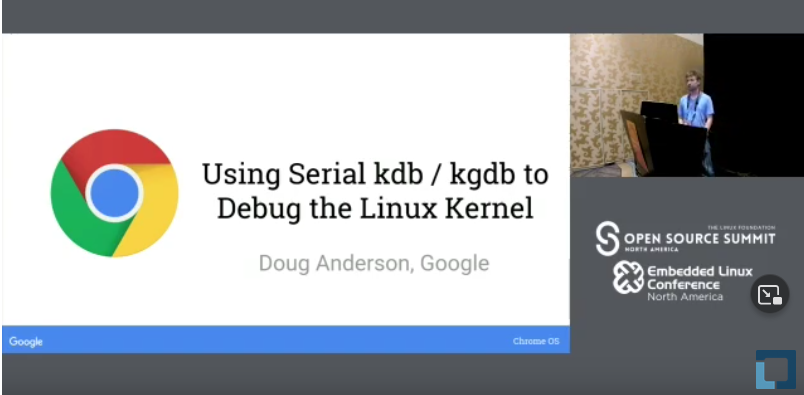
\includegraphics[height=0.5\textheight]{slides/debugging-kernel-debugging/kgdb_conf.png}
  \end{center}
\end{frame}

\subsection{crash}

\begin{frame}
  \frametitle{{\em crash}}
  \begin{itemize}
    \item {\em crash} is a CLI tool allowing to investigate kernel (dead or
      alive!)
    \begin{itemize}
      \item Uses /dev/mem or /proc/kcore on live systems
      \item Requires \kconfigval{CONFIG_STRICT_DEVMEM}{n}
    \end{itemize}
    \item Can use a coredump generated using kdump, kvmdump, etc.
    \item Based on \code{gdb} and provides many specific commands to inspect the
      kernel state.
    \begin{itemize}
      \item Stack traces, dmesg (\code{log}), memory maps of the processes,
            irqs, virtual memory areas, etc.
    \end{itemize}
    \item Allows examining all the tasks that are running on the system.
    \item Hosted at \url{https://github.com/crash-utility/crash}
  \end{itemize}
\end{frame}

\begin{frame}[fragile]
  \frametitle{{\em crash} example}
  \begin{itemize}
    \begin{block}{}
      \begin{minted}[fontsize=\tiny]{console}
$ crash vmlinux vmcore
[...]
    TASKS: 75
NODENAME: buildroot
  RELEASE: 5.13.0
  VERSION: #1 SMP PREEMPT Tue Nov 15 14:42:25 CET 2022
  MACHINE: armv7l  (unknown Mhz)
  MEMORY: 512 MB
    PANIC: "Unable to handle kernel NULL pointer dereference at virtual address 00000070"
      PID: 127
  COMMAND: "watchdog"
    TASK: c3f163c0  [THREAD_INFO: c3f00000]
      CPU: 1
    STATE: TASK_RUNNING (PANIC)

crash> mach
    MACHINE TYPE: armv7l
     MEMORY SIZE: 512 MB
            CPUS: 1
 PROCESSOR SPEED: (unknown)
              HZ: 100
       PAGE SIZE: 4096
KERNEL VIRTUAL BASE: c0000000
KERNEL MODULES BASE: bf000000
KERNEL VMALLOC BASE: e0000000
KERNEL STACK SIZE: 8192
      \end{minted}
    \end{block}
  \end{itemize}
\end{frame}

\subsection{Post-mortem analysis}

\begin{frame}
  \frametitle{Kernel crash post-mortem analysis}
  \begin{itemize}
    \item Sometimes, accessing the crashed system is not possible or the system
          can't stay offline while waiting to be debugged
    \item Kernel can generate crash dumps (a {\em vmcore} file) to a remote
          location, allowing to quickly restart the system while still
          be able to perform post-mortem analysis with GDB.
    \item This feature relies on {\em kexec} and {\em kdump} which will
          boot another kernel as soon as the crash occurs right after dumping the
          {\em vmcore} file.
    \begin{itemize}
      \item The {\em vmcore} file can be saved on local storage, via SSH, FTP etc.
    \end{itemize}
  \end{itemize}
\end{frame}

\begin{frame}[fragile]
  \frametitle{kexec \& kdump (1/2)}
  \begin{itemize}
    \item On panic, the kernel kexec support will execute a "dump-capture
      kernel" directly from the kernel that crashed
    \begin{itemize}
      \item Most of the time, a specific dump-capture kernel is compiled
        for that task (minimal config with specific initramfs/initrd)
    \end{itemize}
    \item {\em kexec} system works by saving some RAM for the kdump kernel
      execution at startup
    \begin{itemize}
      \item \code{crashkernel} parameter should be set to specify the crash
            kernel dedicated physical memory region
    \end{itemize}
    \item {\em kexec-tools} are then used to load dump-capture kernel into
      this memory zone using the \code{kexec} command
    \begin{itemize}
      \item Internally uses the \code{kexec_load} system call
        \manpage{kexec_load}{2}
    \end{itemize}
  \end{itemize}
\end{frame}

\begin{frame}
  \frametitle{kexec \& kdump (2/2)}
  \begin{itemize}
    \item Finally, on panic, the kernel will reboot into the "dump-capture"
      kernel allowing the user to dump the kernel coredump (\code{/proc/vmcore})
      onto whatever media
    \item Additional command line options depends on the architecture
    \item See \kdochtml{admin-guide/kdump/kdump} for more comprehensive
      explanations on how to setup the kdump kernel with \code{kexec}.
    \item Additional user-space services and tools allow to automatically
      collect and dump the vmcore file to a remote location.
    \begin{itemize}
      \item See kdump systemd service and the \code{makedumpfile} tool which
        can also compress the vmcore file into a smaller file (Only for x86,
        PPC, IA64, S390).
      \item \url{https://github.com/makedumpfile/makedumpfile}
    \end{itemize}
  \end{itemize}
\end{frame}

\begin{frame}
  \frametitle{kdump}
  \center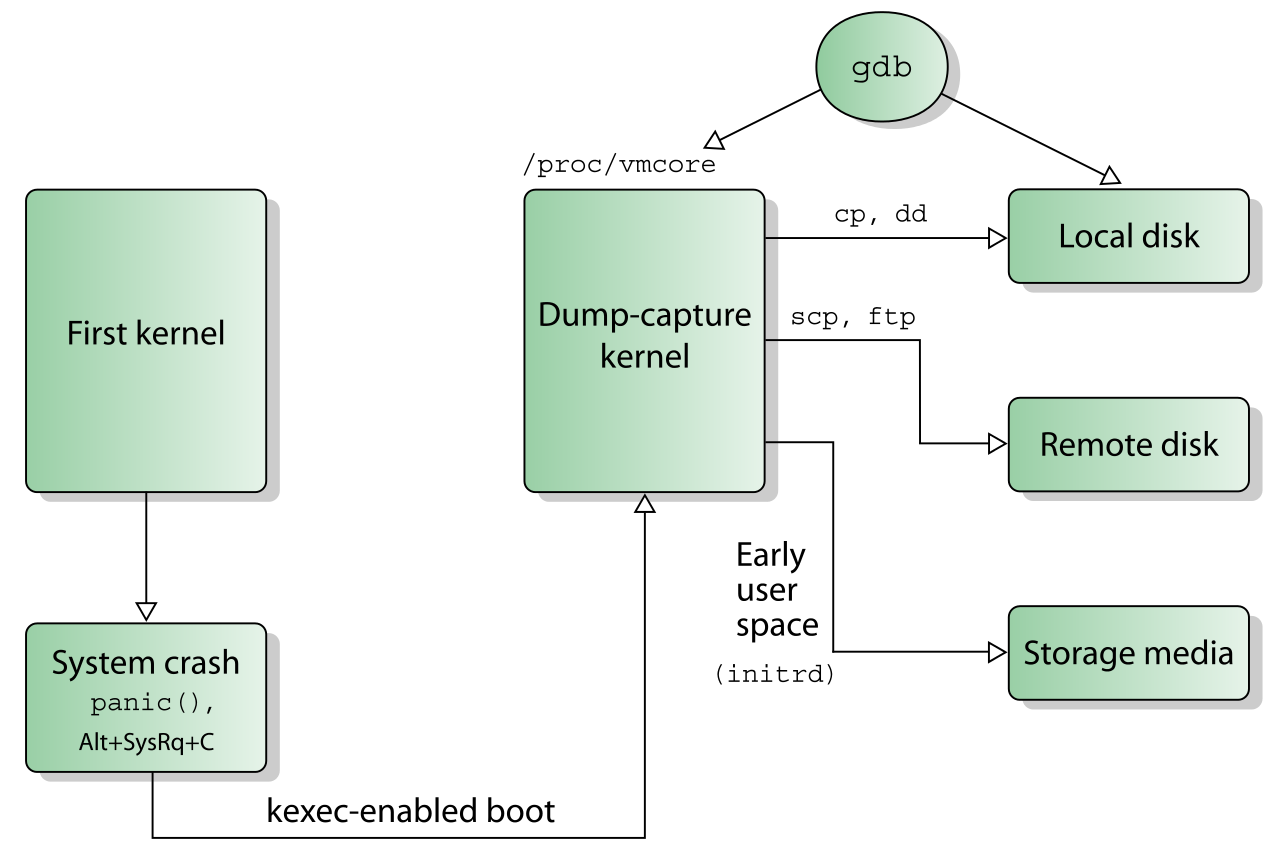
\includegraphics[height=0.8\textheight]{slides/debugging-kernel-debugging/kdump.png}\\
  \tiny Image credits: Wikipedia
\end{frame}

\begin{frame}[fragile]
  \frametitle{kexec config and setup}
  \begin{itemize}
    \item On the standard kernel:
    \begin{itemize}
      \item \kconfigval{CONFIG_KEXEC}{y} to enable KEXEC support
      \item \code{kexec-tools} to provide the \code{kexec} command
      \item A kernel and a DTB accessible by \code{kexec}
    \end{itemize}
    \item On the dump-capture kernel:
    \begin{itemize}
      \item \kconfigval{CONFIG_CRASH_DUMP}{y} to enable dumping a crashed
            kernel
      \item \kconfigval{CONFIG_PROC_VMCORE}{y} to enable \code{/proc/vmcore}
        support
      \item \kconfigval{CONFIG_AUTO_ZRELADDR}{y} on ARM32 platforms
    \end{itemize}
    \item Set the correct \code{crashkernel} command line option:
    \begin{itemize}
      \item \code{crashkernel=size[KMG][@offset[KMG]]}
    \end{itemize}
    \item Load a dump-capture kernel on the first kernel with \code{kexec}:
    \begin{itemize}
      \item \code{kexec --type zImage -p my_zImage --dtb=my_dtb.dtb
        --initrd=my_initrd --append="command line option"}
    \end{itemize}
    \item Then simply wait for a crash to happen!
  \end{itemize}
\end{frame}

\begin{frame}[fragile]
  \frametitle{Going further with kexec \& kdump}
  \begin{itemize}
    \item Presentation from Steven Rostedt about using kexec, kdump and ftrace
          with lot of tips and tricks about using kexec/kdump
    \begin{itemize}
      \item Video: \url{https://www.youtube.com/watch?v=aUGNDJPpUUg}
      \item Slides: \url{https://static.sched.com/hosted_files/ossna2022/c0/Postmortem_%20Kexec%2C%20Kdump%20and%20Ftrace.pdf}
    \end{itemize}
  \end{itemize}
  \vspace{0.1cm}
  \begin{center}
  \center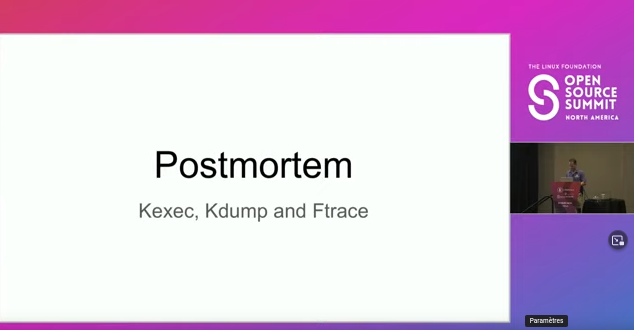
\includegraphics[height=0.5\textheight]{slides/debugging-kernel-debugging/kexec_kdump_ftrace.png}
  \end{center}
\end{frame}

\setuplabframe
{Kernel debugging}
{
  Debugging kernel crashes and driver problems
  \begin{itemize}
    \item Debug locking issues using lockdep
    \item Use kmemleak to detect memory leaks on the system
    \item Analyze an OOPS message
    \item Debug a crash with KGDB
    \item Setup kexec, kdump and extract a kernel coredump
  \end{itemize}
}
